\section{熊野寮概要} \label{sec:abst}
\index{くまのりょう@熊野寮}

		\subsection{基本データ} \label{subsec:data}
		\begin{table}[htbp]
      \begin{tabular}{|l|l|l|}
      \hline
      寮費\index{りょうひ@寮費|seealsopage{維持費}}  & 維持費\index{いじひ@維持費|seealsopage{寮費}}    & 月4,300円(水光熱費込み)。維持費の4,300円への値上げについては以下を参照                    \\
          & 入寮予備金  & 3,000円                                                       \\ \hline
      寮食\index{りょうしょく@寮食}  & 内容     & 基本的に朝昼夕の三食                                                   \\
          & 期間     & 授業期間の平日(土日祝は休み)                \\
          & 食券代\index{りょうしょく@寮食!のねだん@---の値段}    & 朝180円、昼290円、夕420円 \\
          & & (5食分以上のまとめ買いのカードなら朝10円、昼夕は30円引き)         \\ \hline
      連絡先\index{くまのりょう@熊野寮!のれんらくさき@---の連絡先}
       & 住所\index{くまのりょう@熊野寮!のじゅうしょ@---の住所}   & 606--8393 京都府京都市左京区丸太町通川端東入東竹屋町50 京都大学熊野寮                     \\
          & 電話番号   & 075--751--4050 または 075--751--4051                                \\
          & 入寮選考関係\index{にゅうりょう@入寮!にかんするといあわせ@---に関する問い合わせ} & メール:interview@kumano-ryo.com \\
           & & LINE公式アカウント:@109wsqij(入退寮選考委員会) \\ \hline
      \end{tabular}
      \end{table}
    \begin{tcolorbox}[colback=white, colbacktitle=gray!30!white, coltitle=black, title=2022年4月からの寮費200円値上げについて,breakable]
      \setlength{\parindent}{1zw}
      \small{このたび熊野寮自治会では、京都大学からの不当な干渉によって財政状況が不安定となり、維持費(寮費)を値上げするという苦渋の決断をするに至りました。
      
      熊野寮自治会は学生の金銭的負担を軽減するため、食堂調理員を全て大学雇用に戻し、従来通りに全厨房員の人件費を支払うことを大学当局に要求していきます。(※)
      
      寮自治会の財政状況として、京都大学が1979年より長らく食堂調理員\index{ちゅうぼういん@厨房員}の人件費不払い(雇用拒否)の方針を採っているために、寮生がその肩代わりとして人件費を不当に負担させられており、寮運営が困難な状況がこれまで続いていました。そして2021年の夏、京都大学が自販機業者に圧力をかけたことにより、寮自治会が契約していた寮内自販機が強制解約され、寮の財政はさらに悪化しました。この自販機はそもそも営利目的ではなく、寮生の福利厚生を充実させるために、熊野寮自治会が自治権の範囲内で2008年より設置したものです。売値は全て100円以下で、利用者である寮生個人にとっても経済性・利便性が高いうえに、その売上げは寮自治会の財源となって寮生の福利厚生に還元されてきました。
      長らく食堂人件費の負担を強いられてきたうえに、今回の自販機強制解約によって、寮自治会は維持費の値上げをするに至りました。
      
      \noindent(※)京都大学と熊野寮自治会の合意について\\

      現在、平島学生担当副学長と熊野寮自治会の間に結ばれている確約\index{かくやく@確約}においても、「過去に熊野寮食堂の食堂労働者を削減した事実を認める」こと、および「寮内労働者の雇用形態について本来ならば全員大学雇いが望ましいことを認め、その労働環境・労働条件に関しては改善に努める」ことが確認されています。(確約全文は当パンフ\pageref{page:確約}ページを参照)}

    \end{tcolorbox}


		\subsection{建物概略}
    \index{くまのりょう@熊野寮!のたてもの@---の建物}
		\begin{description}
		\item 居室のあるA棟、B棟、C棟(4階建て)と食堂(平屋)。全て鉄筋コンクリート。
		\item 築約60年、各階11部屋(例外あり)、総部屋数127
		\item[定員] 422名
		\item[居室] A棟16畳、B棟18畳(定員4名)、C棟8畳(定員2名)。C棟は3部屋を6人で用いるなどしています。\index{きょしつ@居室}\index{へや@部屋|see{談話室, 居室}}
		\item[備品] 事務机、椅子、本棚、二段ベッド\index{べっど@ベッド}、クローゼット\index{きょしつ@居室!のびひん@---の備品}
		\end{description}

    \subsection{ブロック}
    \noindent ブロック〈block〉各棟のフロアを基準に構成されるグループ。ブロック会議を行ったり炊事当番や事務室当番などの仕事が割り振られたりするほか、娯楽のためのイべントを内部で催すことがある。\\
    「—はどこ?」「—の後輩」「同部屋同—」

		\subsection{共同設備}

    \renewcommand{\arraystretch}{1.2}
    \vspace{-8mm}
    \begin{table}[htbp]
      \begin{tabular}{lp{43zw}}
        
        \textbf{居室内}  & 冷蔵庫\index{れいぞうこ@冷蔵庫}・テレビ\index{てれび@テレビ}・電気ケトル・炊飯器などは上回生が持っていたり、部屋で受け継がれていたりする場合がある。 防災上、石油ストーブ\index{だんぼうきぐ@暖房器具}は禁止。 寮内は屋上含め全面禁煙\index{たばこ@たばこ|seealsopage{喫煙所}}。 喫煙所\index{きつえんじょ@喫煙所}が玄関脇にある。水道はない。\index{きょしつ@居室!のびひん@---の備品}
        \\  
        \textbf{談話室}  & おおむね各階に設けられた十数畳の部屋。 各階の集会場兼遊戯室となる。 使用状況は階によって様々だが、たいてい漫画・ゲームなどが置いてある。\index{だんわしつ@談話室}    \\ 
        \textbf{炊事場}  & 各階にある。 ガスコンロ・ガス湯沸かし器・流し・鏡などがある。\index{すいじば@炊事場}\index{だいどころ@台所|see{炊事場}}
        \\ 
        \textbf{洗濯機}  & 各階にある。 各棟屋上\index{おくじょう@屋上}には物干し場と乾燥機がある。 \index{せんたく@洗濯|seealsopage{屋上}}        
        \\ 
        \textbf{トイレ}  & 各階にある。 水洗トイレ。 和・洋式どちらもある。 B棟一階には多目的トイレがある。C棟二階にはオールジェンダートイレがある。\index{といれ@トイレ}                             \\ 
        \textbf{食堂}   & 栄養士さんが考えたバランスのとれた食事を、日替わりで楽しめる。 食堂内には生協の自動販売機、製氷機、電子レンジがある。 卓球台も置いてある。 食堂はコンパなど多くの催し物に使われる。\index{しょくどう@食堂}    \\ 
        \textbf{事務室}  & 維持費の支払い、来客の対応などをする。 新聞各紙(京都・読売・朝日・毎日・日経) を閲覧できる。 ここでは常時寮生が事務室当番\index{じむしつ@事務室!とうばん@---当番|seealsopage{炊事当番}}として電話の取次ぎや、郵便物の管理を行っている。\index{じむしつ@事務室}     \\ 
        \textbf{シャワー} & A棟一階には男女別のシャワー個室があり、男子6基、女子2基ある。 料金は3分10円のプリペイドカード式。 ドライヤー\index{どらいやあ@ドライヤー}もある。\index{しゃわー@シャワー}\index{ふろ@風呂|see{シャワー}}
        \\ 
        \textbf{ロビー}  & 食堂に準ずる交流の場。 コンパなどに利用される。\index{ろびー@ロビー}\index{げんかん@玄関|see{ロビー}}
             \\ 
        \textbf{音楽室}  & B棟地下にある、スタジオ兼ライブハウス。\index{おんがくしつ@音楽室} 
            \\ 
        \textbf{硬鉄庵}  & B棟地下にある、分厚い扉に守られた部屋。 警察権力からの防衛に特化している。 \index{こうてつあん@硬鉄庵}
        \\
        \textbf{民青池}  & たまに飛び込む者がいる。寮祭企画・みかん祭り\index{くまのりょうさい@熊野寮祭!きかく@---企画}の開催場所になったりもする。元々は防火用。   \\ 
        \textbf{娯楽}   & 食堂の卓球台、敷地内のバスケットゴール・フットサルコート\index{ふっとさるこーと@フットサルコート}などに加え、部屋で受け継がれているものもある。\index{ごらく@娯楽|seealsopage{ゲーム, 麻雀}}\index{あそび@遊び|see{娯楽}}     \\                                 
    \end{tabular}
  \end{table}

  \renewcommand{\arraystretch}{1.0}
  %表の行の高さをもとに戻す

  %ここに建物の写真か何か入れる 

  \vspace{-5mm}
  \begin{figure}[H]
    \centering
    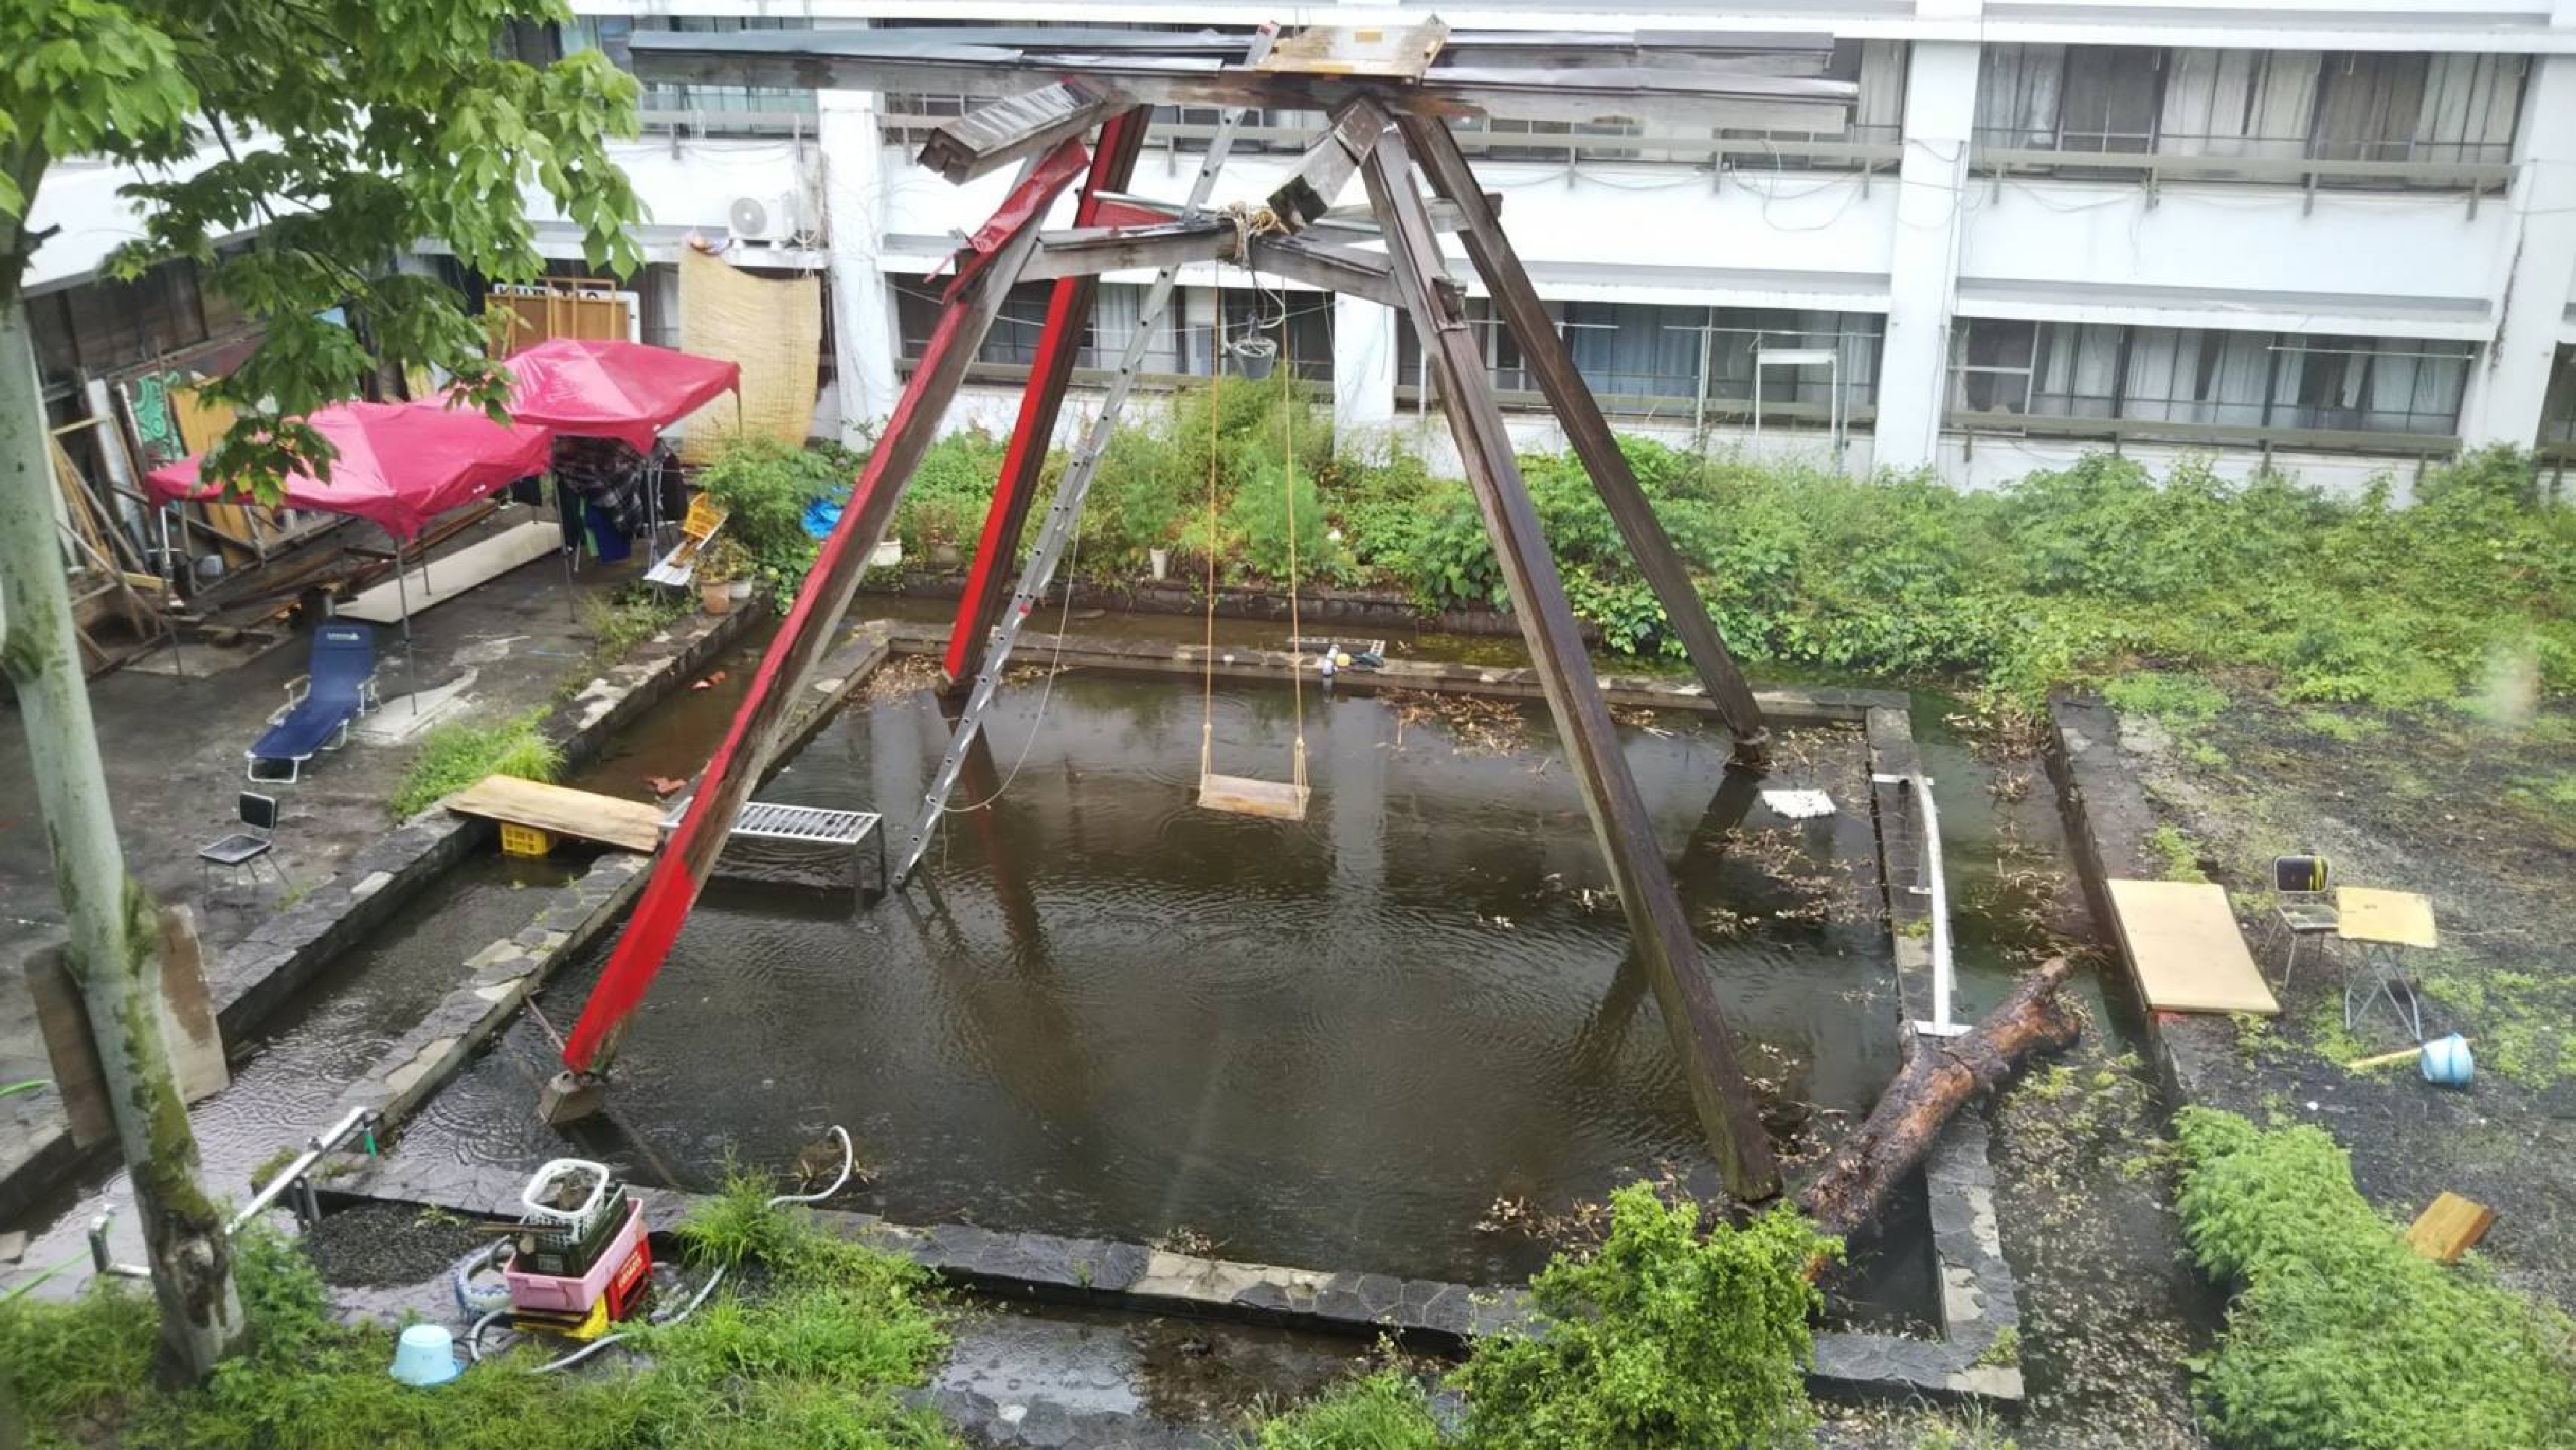
\includegraphics[width=6cm]{gazo/minseike.pdf}
    \caption*{{\small 民青池}}
  \end{figure}





%下は罫線があるバージョンの表
	% 	\begin{table}[htbp]
  %     \begin{tabular}{|lp{43zw}|}
  %       \hline
  %       \textbf{居室内}  & 冷蔵庫・テレビ・電気ケトル・炊飯器などは上回生が持っていたり、部屋で受け継がれていたりする場合がある。 防災上、石油ストーブは禁止。 寮内は屋上含め全面禁煙。 喫煙所が玄関脇にある。水道はない。 \\  \hline
  %       \textbf{談話室}  & おおむね各階に設けられた十数畳の部屋。 各階の集会場兼遊戯室となる。 使用状況は階によって様々だが、たいてい漫画・ゲームなどが置いてある。     \\ \hline
  %       \textbf{炊事場}  & 各階にある。 ガスコンロ・ガス湯沸かし器・流し・鏡などがある。                                                           \\ \hline
  %       \textbf{洗濯機}  & 各階にある。 各棟屋上には物干し場と乾燥機がある。                                                                   \\ \hline
  %       \textbf{トイレ}  & 各階にある。 水洗トイレ。 和・洋式どちらもある。 B棟一階には多目的トイレがある。C棟二階にはオールジェンダートイレがある。                             \\ \hline
  %       \textbf{食堂}   & 栄養士さんが考えたバランスのとれた食事を、日替わりで楽しめる。 食堂内には自動販売機、製氷機、電子レンジがある。 卓球台も置いてある。 食堂はコンパなど多くの催し物に使われる。    \\ \hline
  %       \textbf{事務室}  & 維持費の支払い、来客の対応などをする。 新聞各紙(京都・読売・朝日・毎日・日経) を閲覧できる。 ここでは常時寮生が事務室当番として電話の取次ぎや、郵便物の管理を行っている。     \\ \hline
  %       \textbf{シャワー} & A棟一階には男女別のシャワー個室があり、男子6基、女子2基ある。 料金は3分10円のプリペイドカード式。 ドライヤーもある。                              \\ \hline
  %       \textbf{ロビー}  & 食堂に準ずる交流の場。 コンパなどに利用される。                                                                    \\ \hline
  %       \textbf{音楽室}  & B棟地下にある、スタジオ兼ライブハウス。                                                                        \\ \hline
  %       \textbf{硬鉄庵}  & B棟地下にある、分厚い扉に守られた部屋。 警察権力からの防衛に特化している。                                                      \\ \hline
  %       \textbf{民青池}  & たまに飛び込む者がいる。 寮祭企画・みかん祭りの開催場所になったりもする。元々は防火用。   \\ \hline
  %       \textbf{娯楽}   & 食堂の卓球台、敷地内のバスケットゴール・フットサルコートなどに加え、部屋で受け継がれているものもある。        \\ \hline                                
  %   \end{tabular}
  % \end{table}

%     \begin{figure}[h]
%  	\begin{flushleft}
%	\includegraphics[scale=0.3]%{muc.pdf}
%	\end{flushleft}
%	\end{figure}